%%%%%%%%%%%%%%%%%%%%%%%%%%%%%%%%%%%%%%%%%%%%%%%%%%%%%%%%%%%%%%%%%%%%%%%%%%%%%%%%
%   Precision Following Test Figures
%%%%%%%%%%%%%%%%%%%%%%%%%%%%%%%%%%%%%%%%%%%%%%%%%%%%%%%%%%%%%%%%%%%%%%%%%%%%%%%%

\chapter{Precision Following Test Figures} \label{app:precisionresults}


\begin{figure}[ht] \centering
    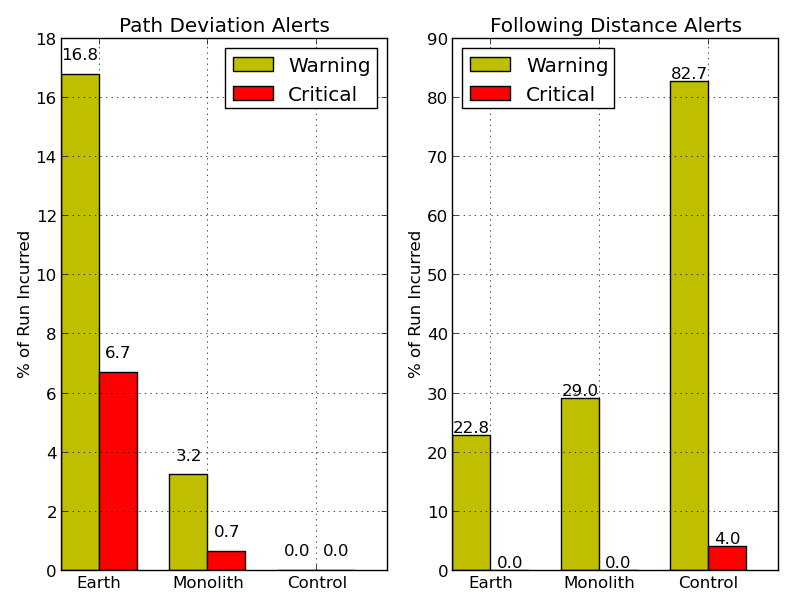
\includegraphics[width=6in]{./figs/precision_following_alert_percents.png}
    \caption{Percentages of runs from Figs.~\ref{fig:precisionresults_earth}, \ref{fig:precisionresults_monolith}, and \ref{fig:precisionresults_control} for which alerts were incurred}
    \label{fig:precision_alerts}
\end{figure}
\begin{figure}[ht] \centering % good.
    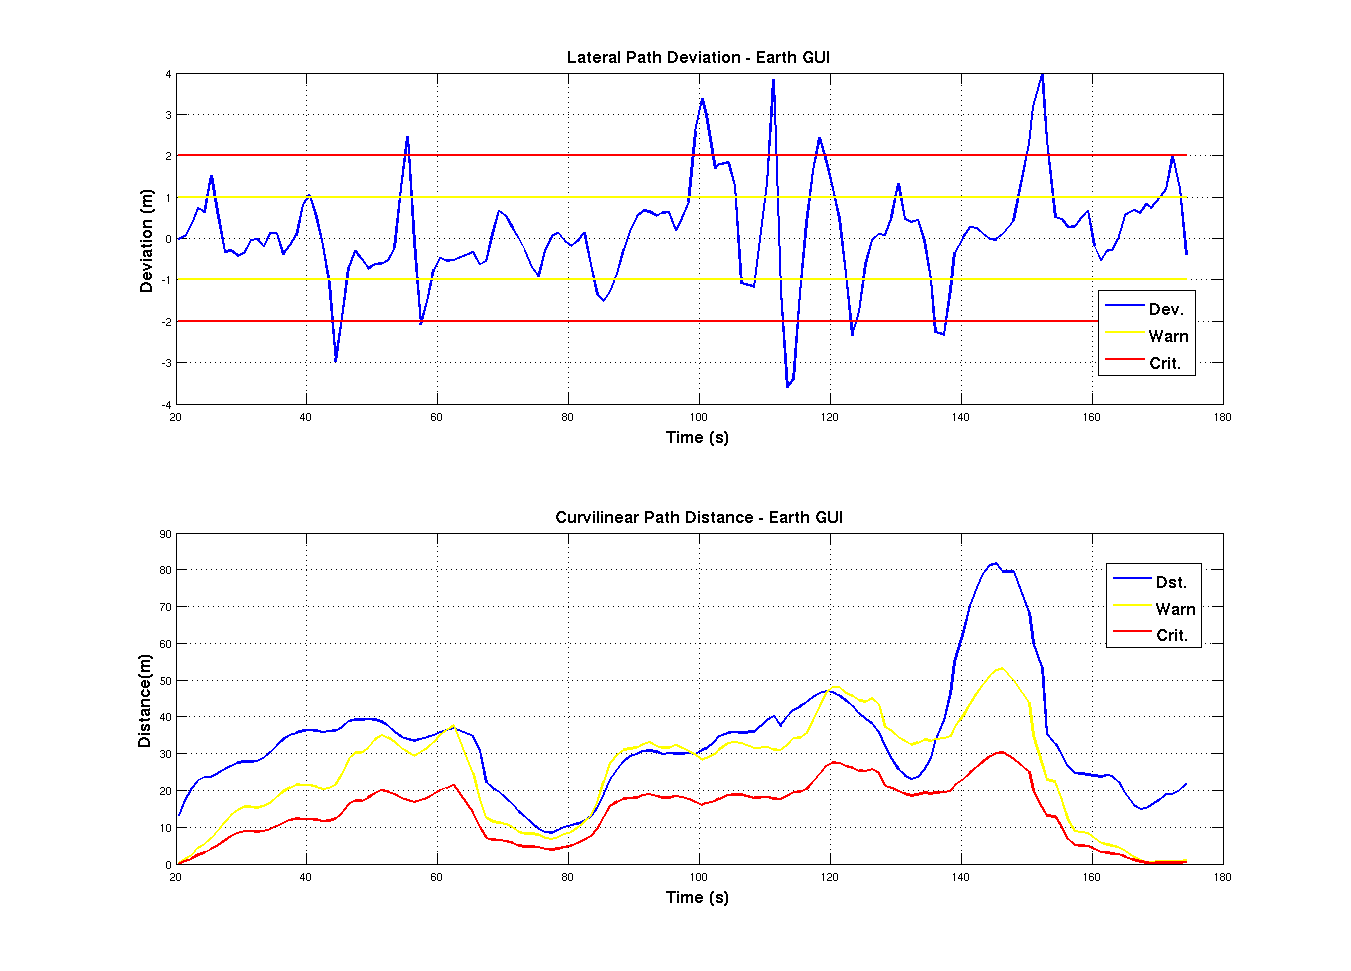
\includegraphics[width=6in]{./figs/precision_following_results_dst_dev_earth.png}
    \caption{Best run of the precision following test using the Earth GUI} \label{fig:precisionresults_earth}
\end{figure}
\begin{figure}[ht] \centering % good.
    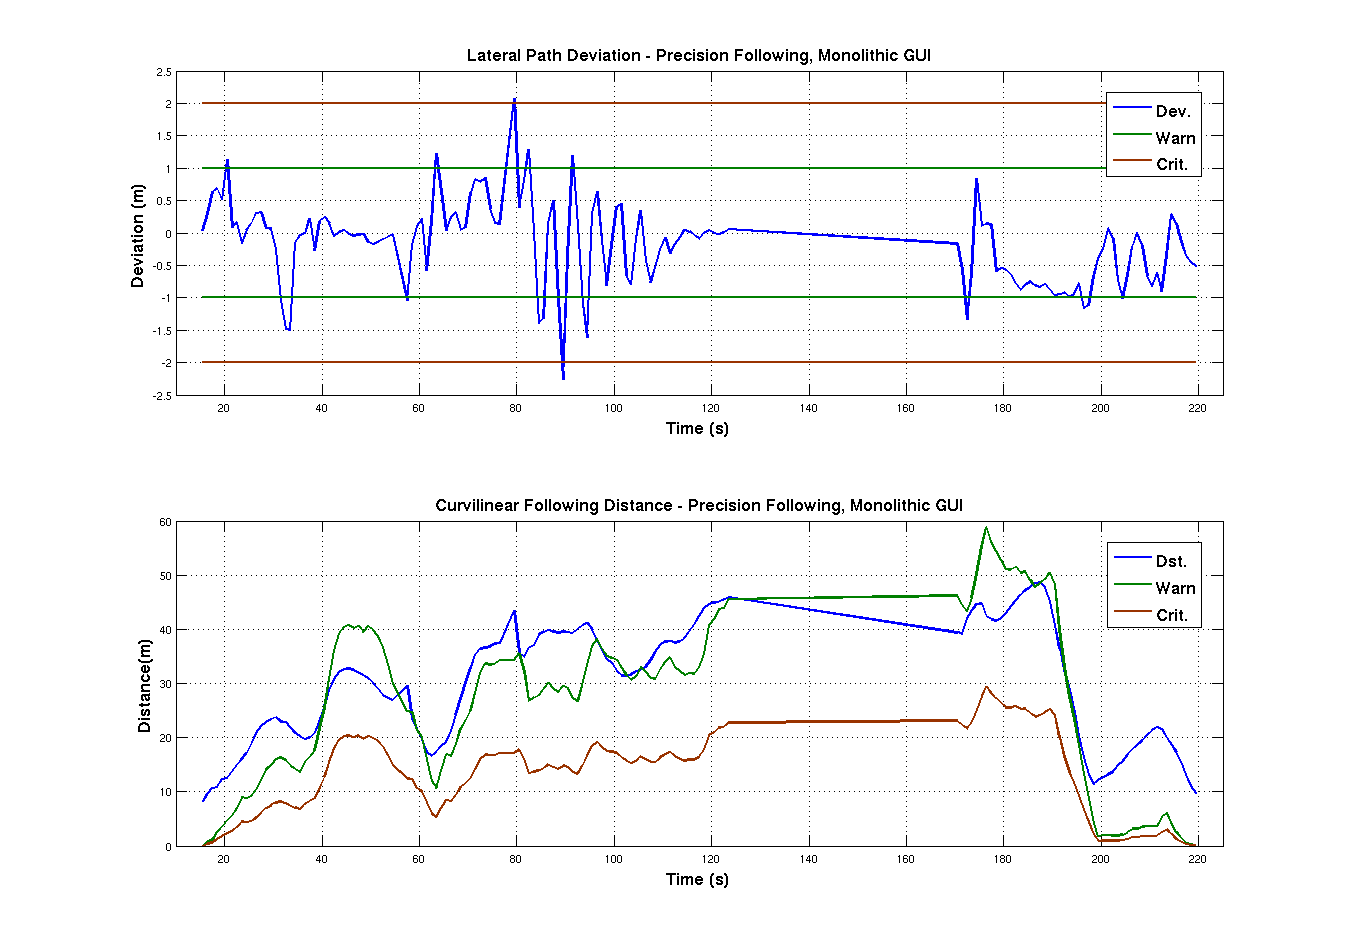
\includegraphics[width=6in]{./figs/precision_following_results_dst_dev_monolith.png}
    \caption{Best run of the precision following test using the monolithic GUI} \label{fig:precisionresults_monolith}
\end{figure}
\begin{figure}[ht] \centering % good.
    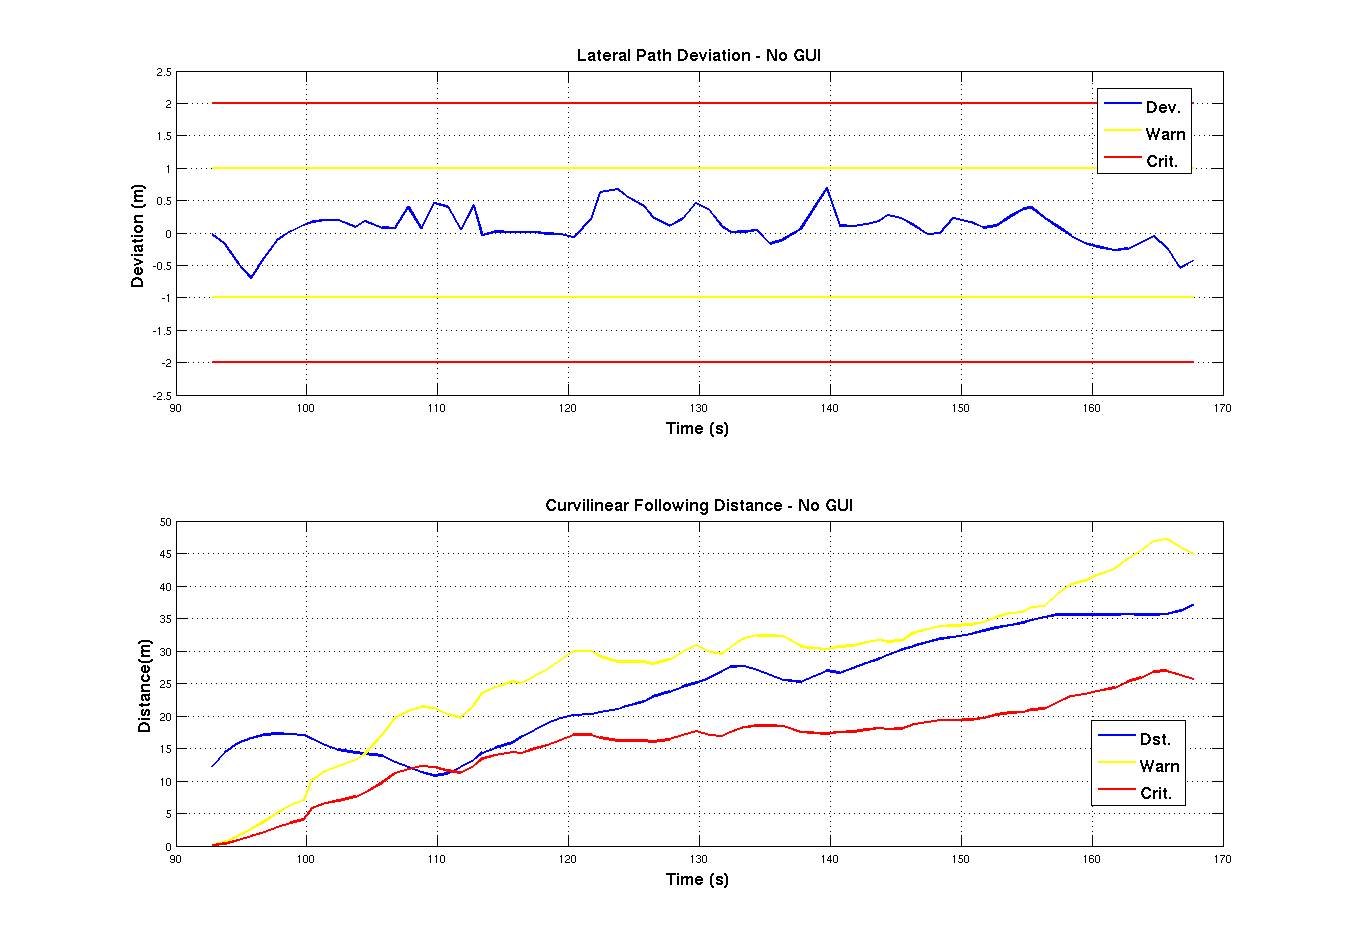
\includegraphics[width=6in]{./figs/precision_following_results_dst_dev_control.png}
    \caption{Best run of the precision following test using no GUI} \label{fig:precisionresults_control}
\end{figure}
\begin{figure}[ht] \centering % good.
    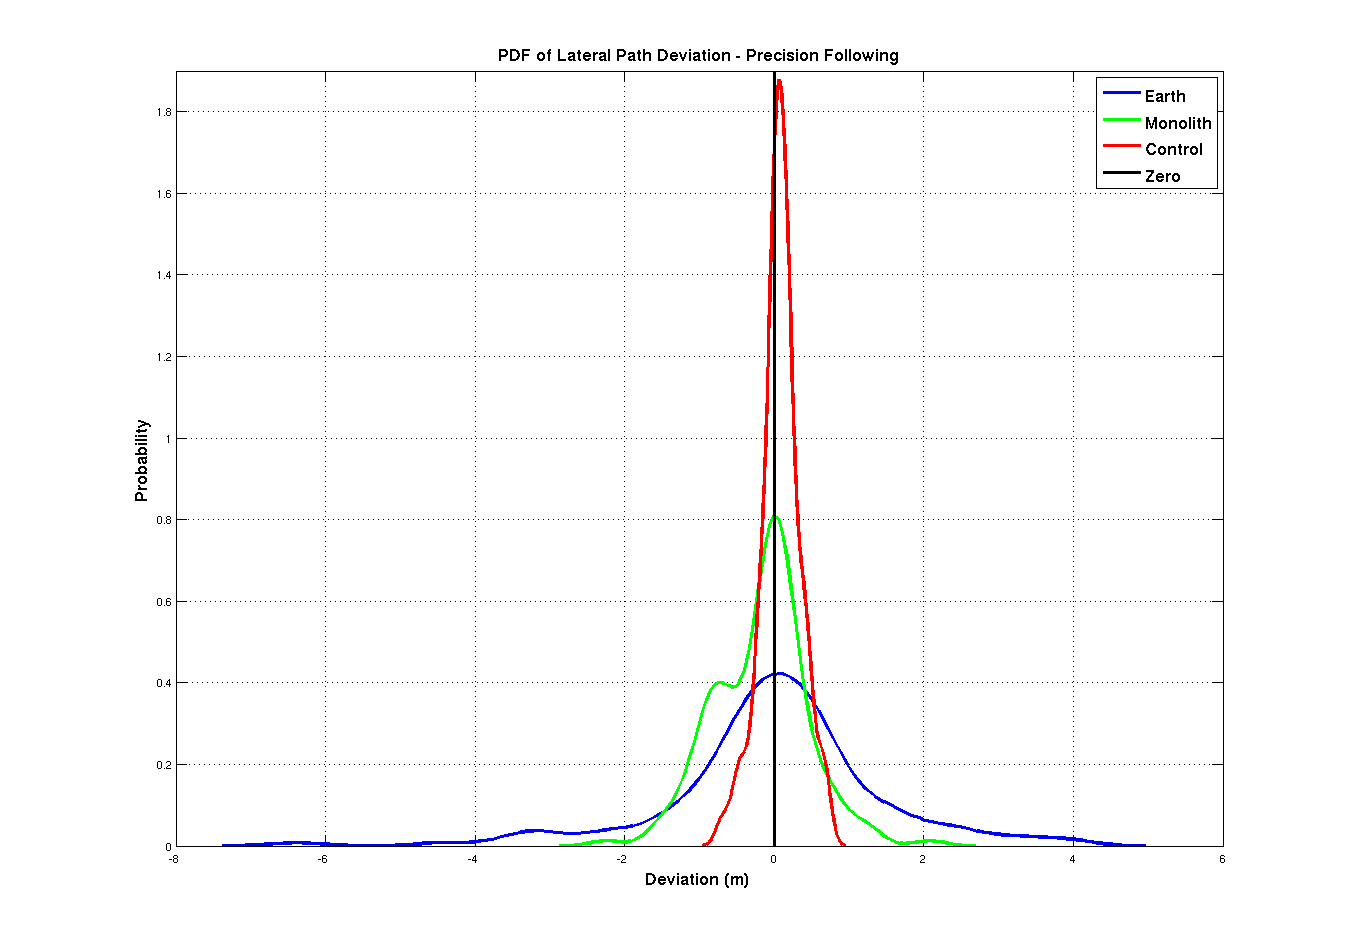
\includegraphics[width=6in]{./figs/precision_following_dev_pdf.png}
    \caption{Comparison of smoothed deviation distributions for the precision following test} \label{fig:precision_dev_dist}
\end{figure}
\begin{figure}[ht] \centering % good.
    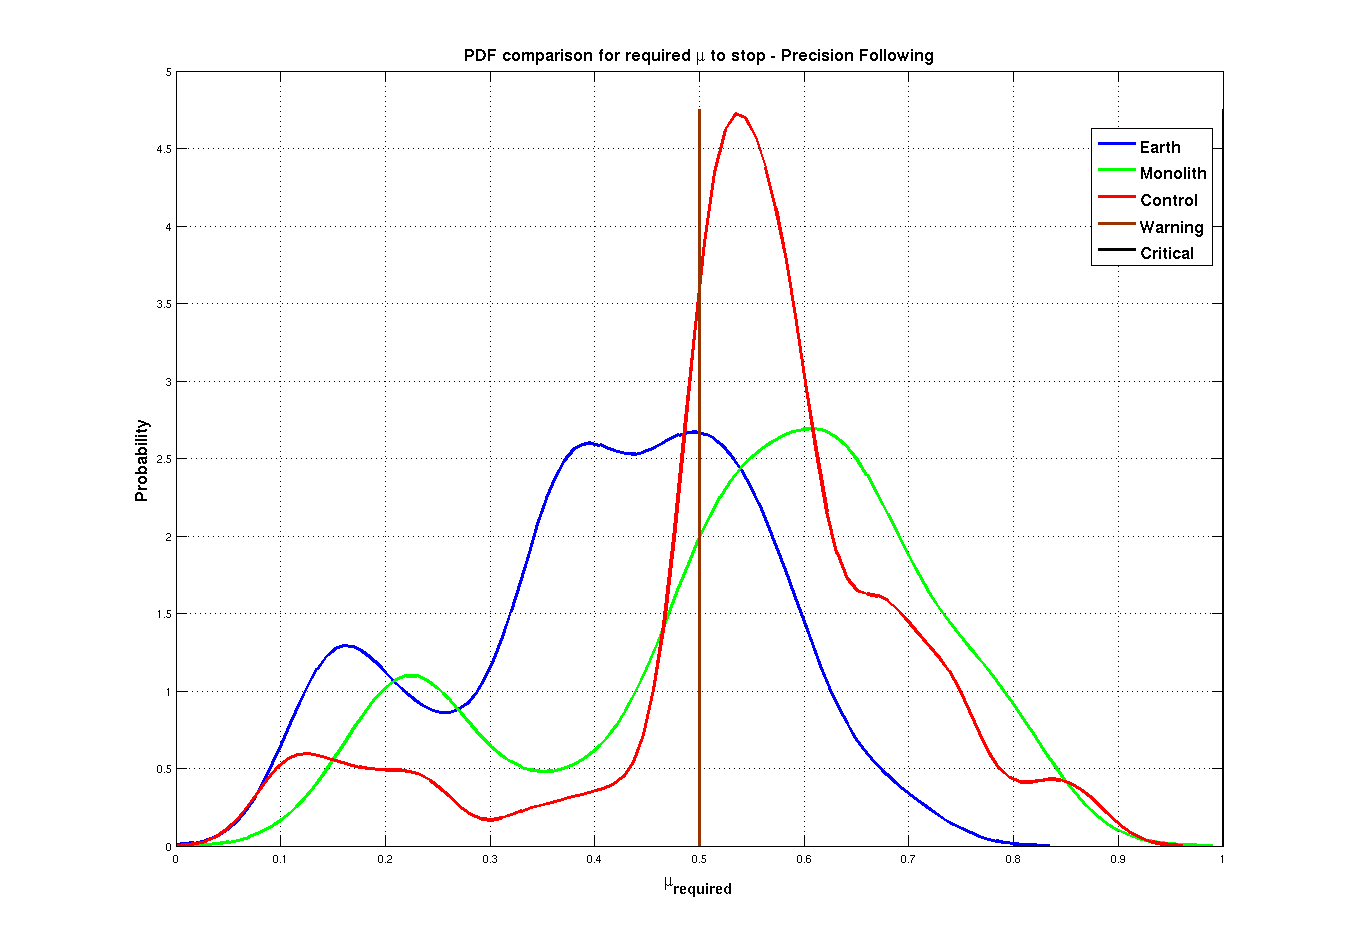
\includegraphics[width=6in]{./figs/precision_following_mu_distribution.png}
    \caption{Comparison of smoothed $\mu_{required}$ distributions for the precision following test} \label{fig:precision_mu_dist}
\end{figure}


%%%%%%%%%%%%%%%%%%%%%%%%%%%%%%%%%%%%%%%%%%%%%%%%%%%%%%%%%%%%%%%%%%%%%%%%%%%%%%%%
%   Zero Landmark Test Figures
%%%%%%%%%%%%%%%%%%%%%%%%%%%%%%%%%%%%%%%%%%%%%%%%%%%%%%%%%%%%%%%%%%%%%%%%%%%%%%%%

\chapter{Zero Landmark Test Figures} \label{app:zeroresults}


\begin{figure}[ht] \centering
    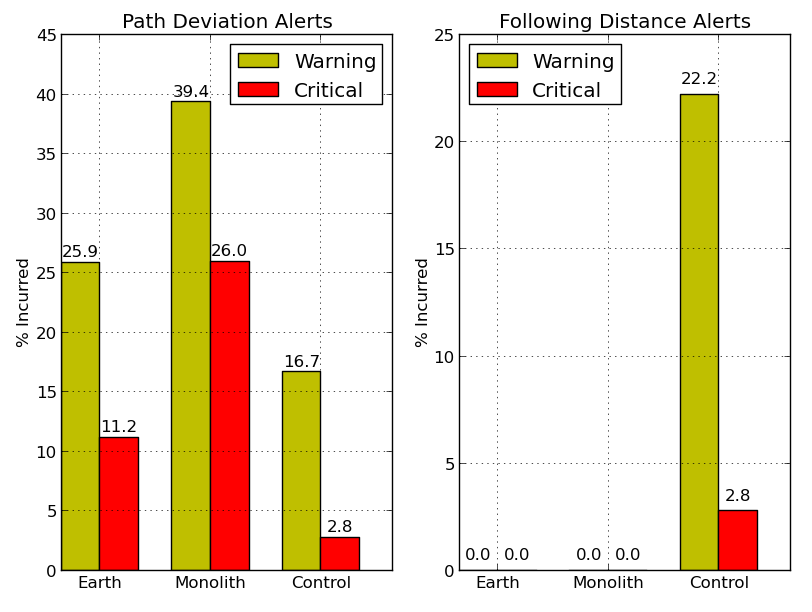
\includegraphics[width=6in]{./figs/zero_landmark_alert_percents.png}
    \caption{Percentages of runs from Figs.~\ref{fig:zeroresults_earth}, \ref{fig:zeroresults_monolith}, and \ref{fig:zeroresults_control} for which alerts were incurred}
    \label{fig:zero_alerts}
\end{figure}
\begin{figure}[ht] \centering
    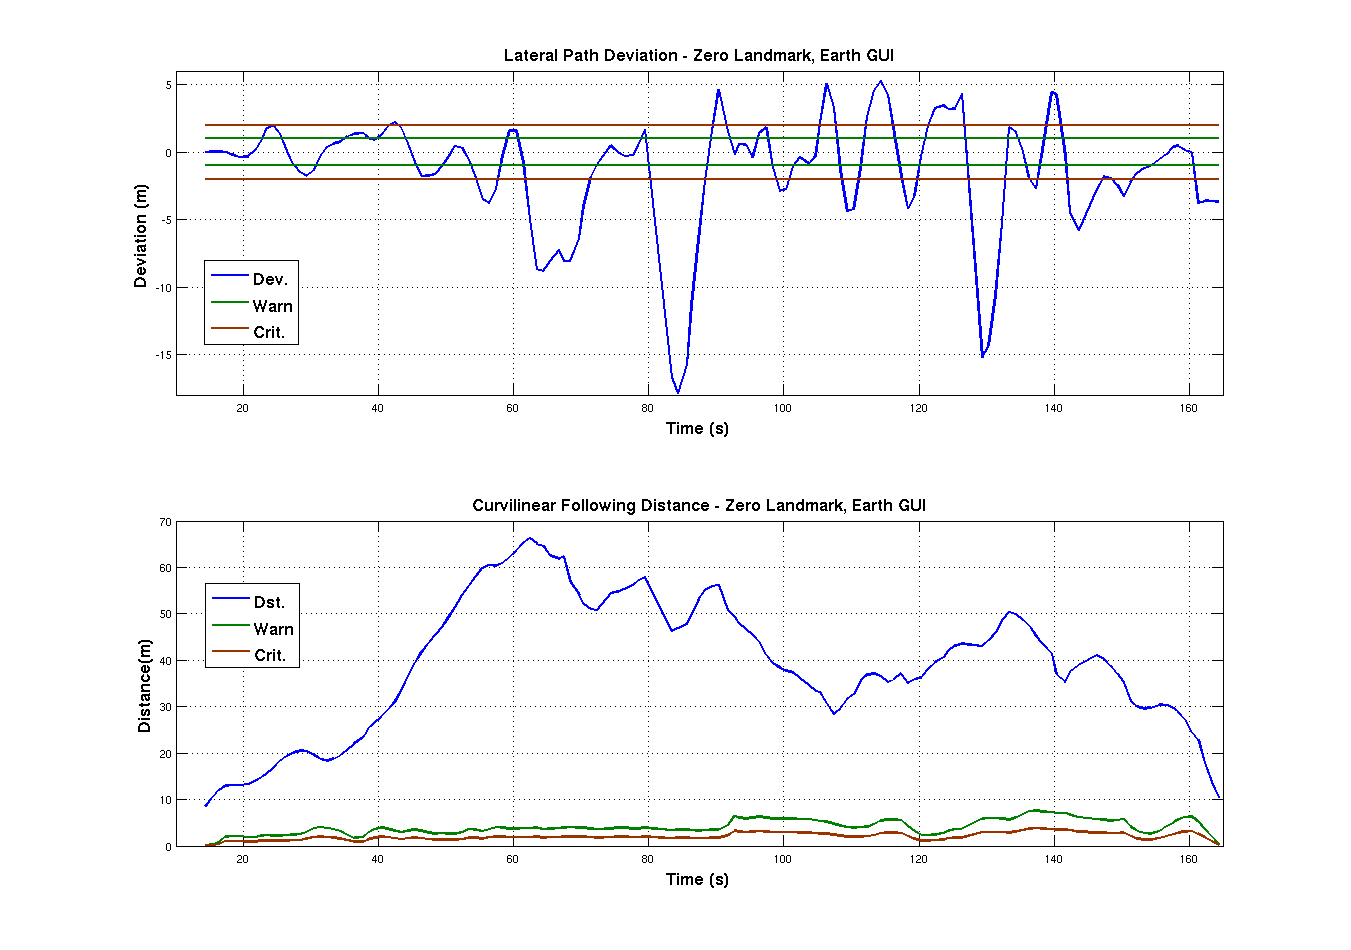
\includegraphics[width=6in]{./figs/zero_landmark_results_dst_dev_earth.png}
    \caption{Best run of the zero landmark test using the Earth GUI} \label{fig:zeroresults_earth}
\end{figure}
\begin{figure}[ht] \centering
    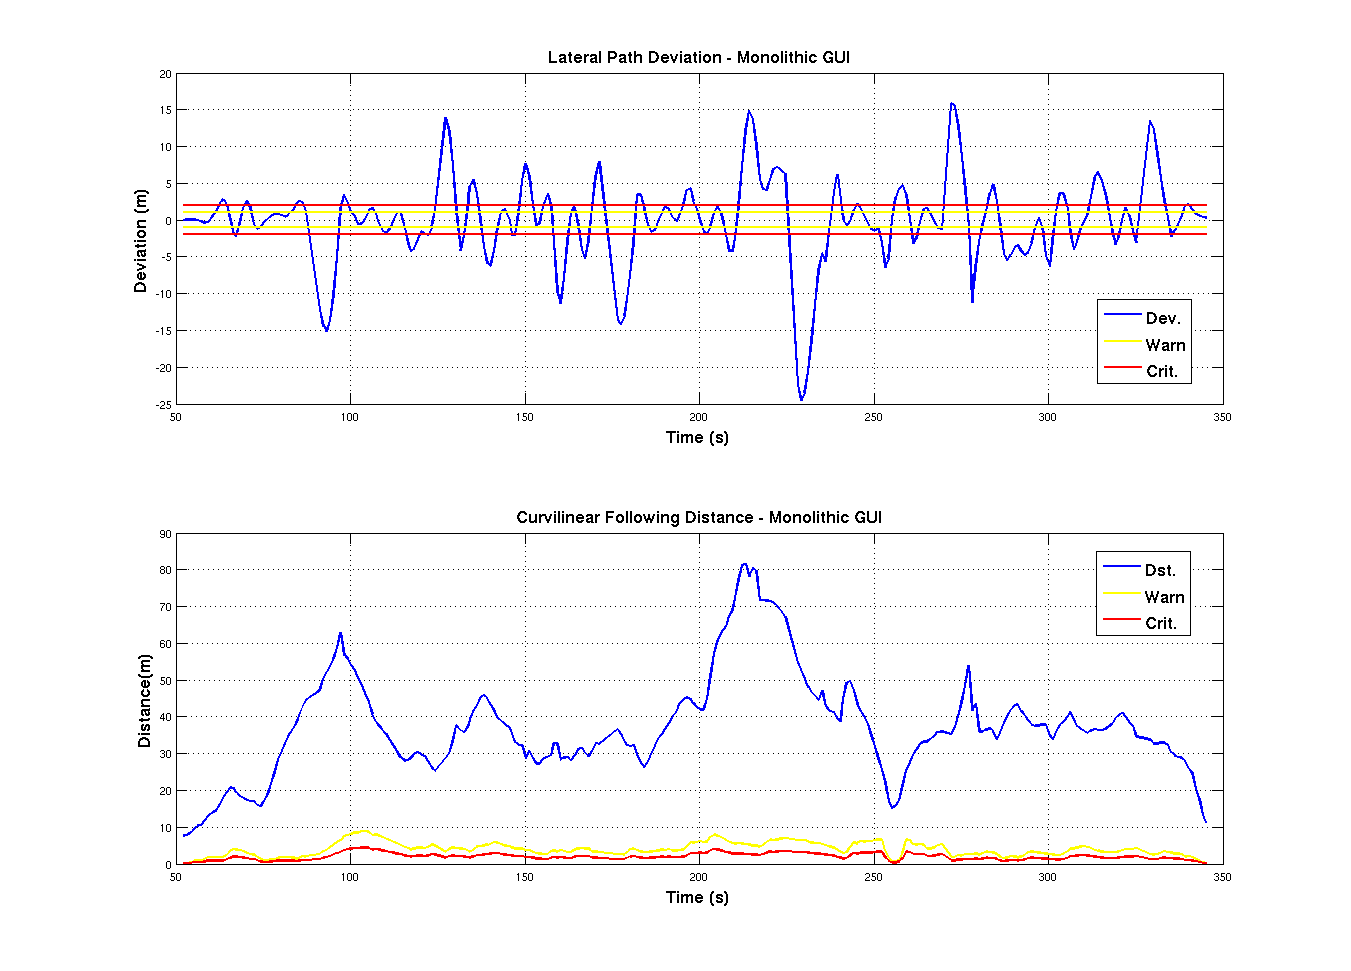
\includegraphics[width=6in]{./figs/zero_landmark_results_dst_dev_monolith.png}
    \caption{Best run of the zero landmark test using the monolithic GUI} \label{fig:zeroresults_monolith}
\end{figure}
\begin{figure}[ht] \centering
    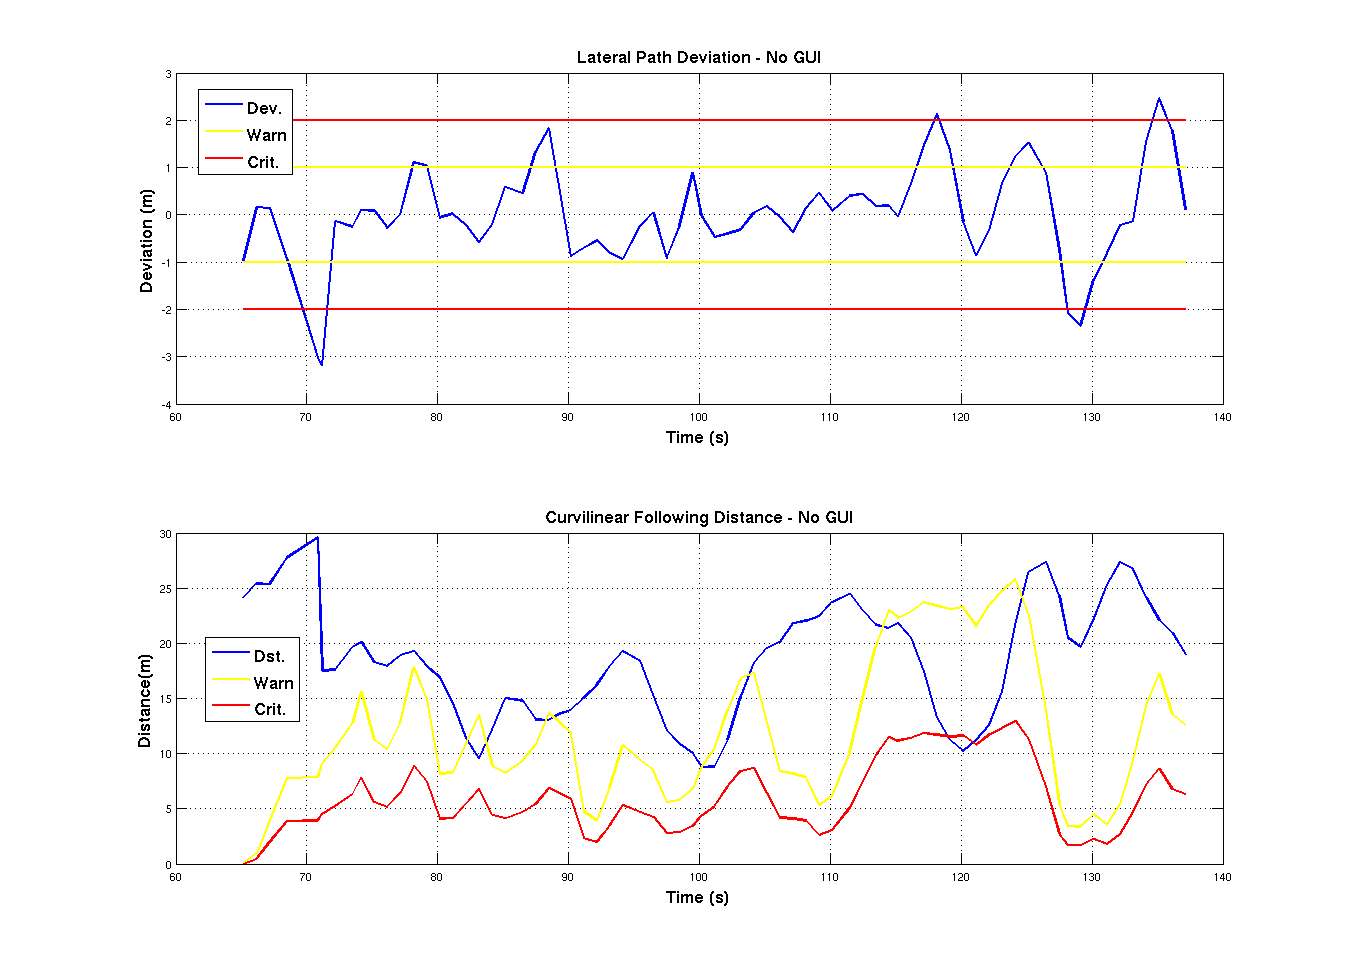
\includegraphics[width=6in]{./figs/zero_landmark_results_dst_dev_control.png}
    \caption{Best run of the zero landmark test using no GUI} \label{fig:zeroresults_control}
\end{figure}
\begin{figure}[ht] \centering % good.
    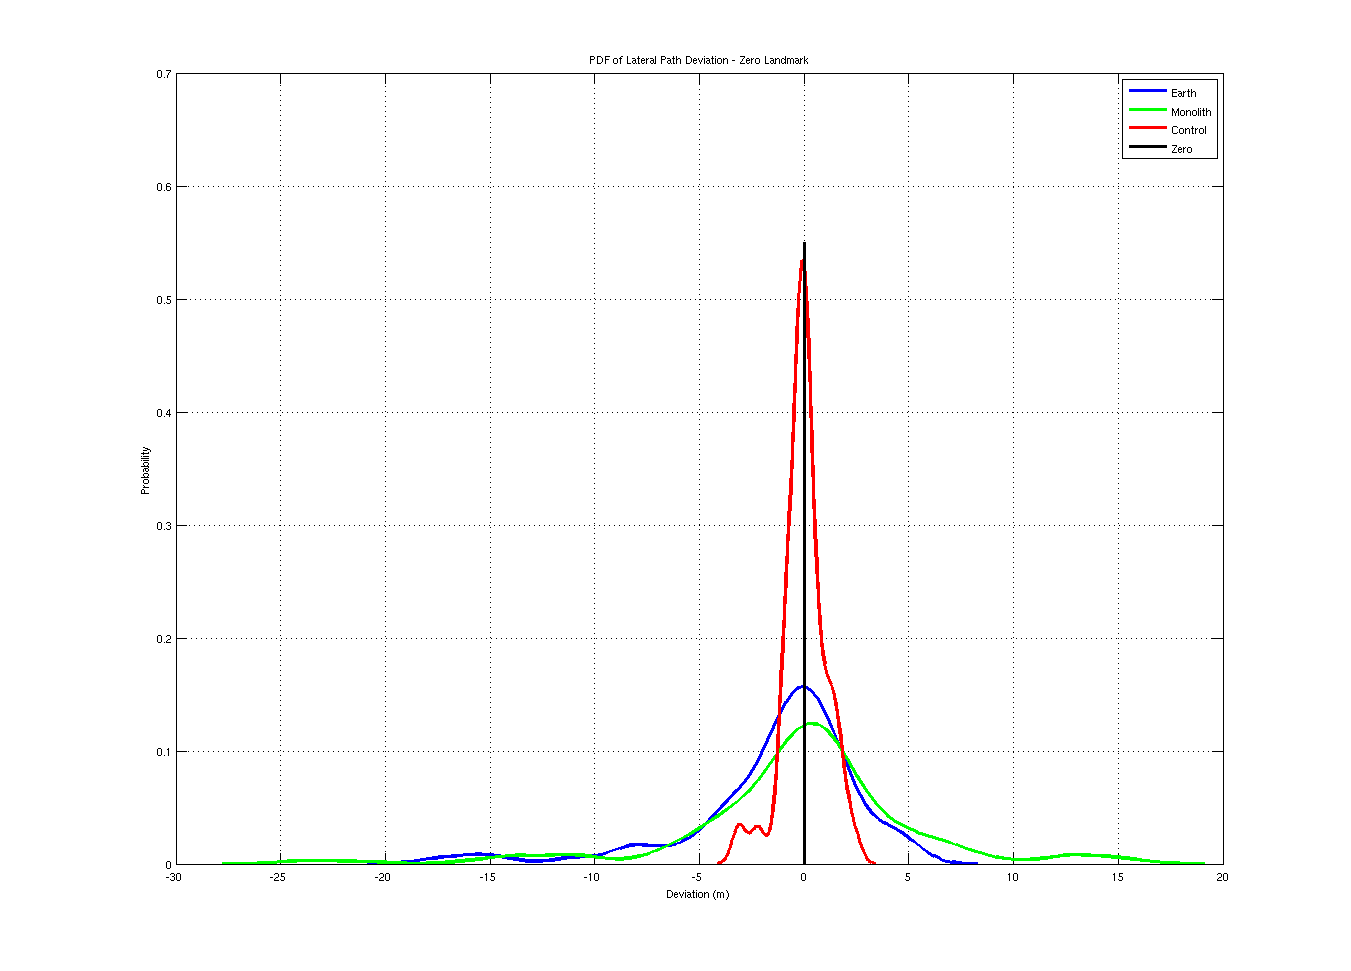
\includegraphics[width=6in]{./figs/zero_landmark_dev_pdf.png}
    \caption{Comparison of smoothed deviation distributions for the zero landmark test} \label{fig:zero_dev_dist}
\end{figure}
\begin{figure}[ht] \centering % good.
    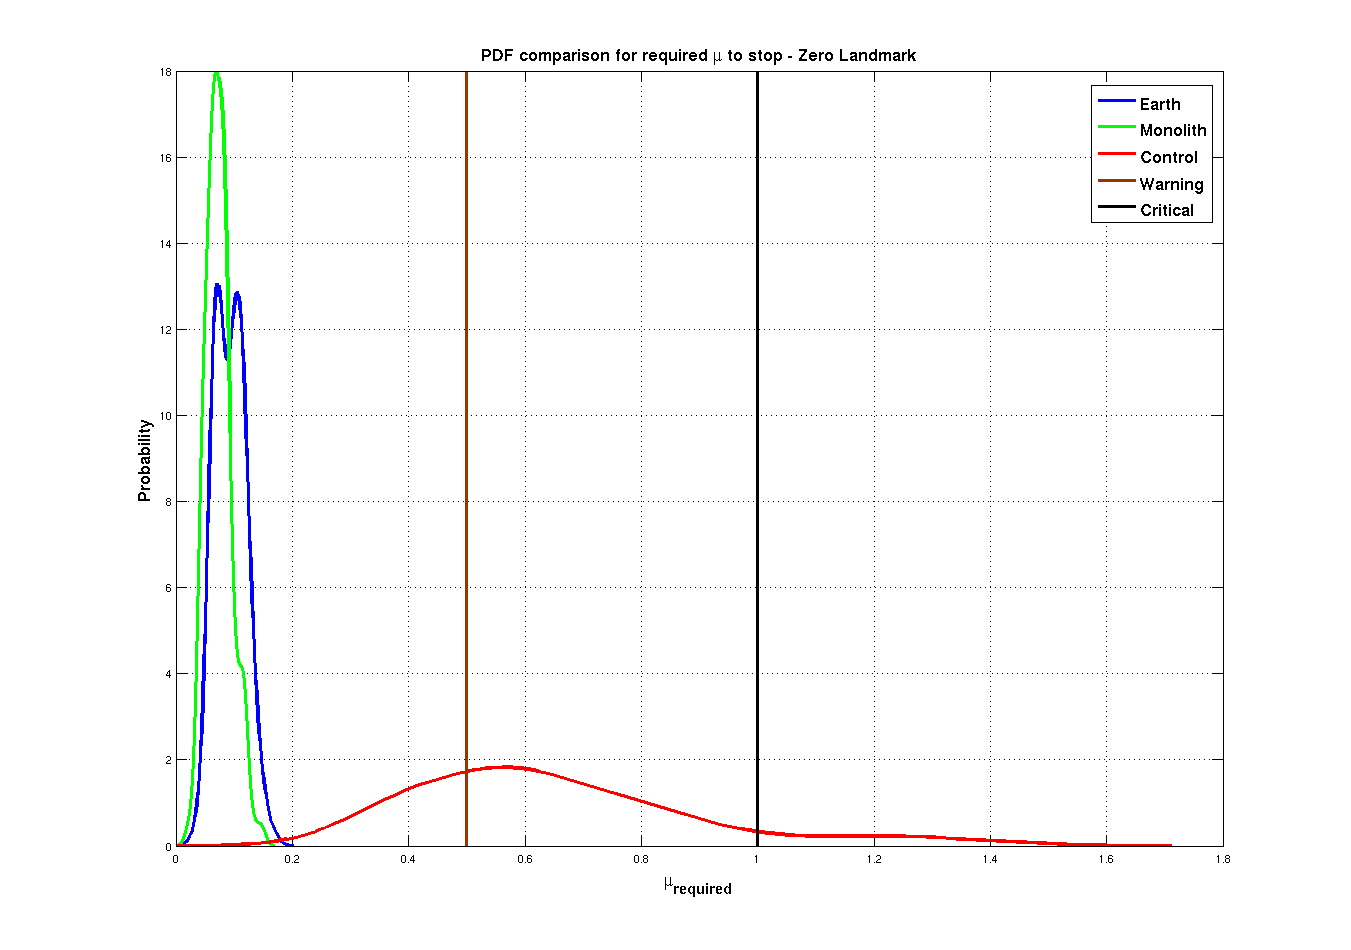
\includegraphics[width=6in]{./figs/zero_landmark_mu_distribution.png}
    \caption{Comparison of smoothed $\mu_{required}$ distributions for the zero landmark test} \label{fig:zero_mu_dist}
\end{figure}
